% ------------------------------------------------------------------
\documentclass[12 pt]{article} % A4 paper set by geometry package below
\pagenumbering{arabic}
\setlength{\parindent}{10 mm}
\setlength{\parskip}{12 pt}

% Nimbus Sans font should be reasonably legible
\usepackage{helvet}
\renewcommand{\familydefault}{\sfdefault}
\usepackage[T1]{fontenc}  % Without this \textsterling produces $

% Section header spacing
\usepackage{titlesec}
\titlespacing\section{0pt}{12pt plus 4pt minus 2pt}{0pt plus 2pt minus 2pt}
\titlespacing\subsection{0pt}{12pt plus 4pt minus 2pt}{0pt plus 2pt minus 2pt}
\titlespacing\subsubsection{0pt}{12pt plus 4pt minus 2pt}{0pt plus 2pt minus 2pt}

\usepackage{amsmath}
\usepackage{amssymb}
\usepackage{graphicx}
\usepackage{verbatim}    % For comment
\usepackage[shortlabels]{enumitem}
\usepackage[paper=a4paper, marginparwidth=0 cm, marginparsep=0 cm, top=2.5 cm, bottom=2.5 cm, left=3 cm, right=3 cm, includemp]{geometry}
\usepackage[pdftex, pdfstartview={FitH}, pdfnewwindow=true, colorlinks=true, citecolor=blue, filecolor=blue, linkcolor=blue, urlcolor=blue, pdfpagemode=UseNone]{hyperref}

\usepackage{framed,color}
\usepackage{fancybox}
\usepackage{varwidth}
\definecolor{shadecolor}{rgb}{1,0.8,0.3}
\usepackage[framemethod=tikz]{mdframed}

% Put module code and last-modified date in footer
\usepackage{fancyhdr}
\pagestyle{fancy}
\fancyhf{}
\renewcommand{\headrulewidth}{0pt}
\cfoot{{\small \thisweek}\hfill \thepage\hfill {\small \moddate}}

% Hopefully address Canvas complaints about pdf tagging
%\usepackage[tagged]{accessibility}
% ------------------------------------------------------------------



% ------------------------------------------------------------------
% Shortcuts
\newcommand{\be}{\ensuremath{\beta} }
\newcommand{\la}{\ensuremath{\lambda} }
\newcommand{\Om}{\ensuremath{\Omega} }
\newcommand{\vev}[1]{\ensuremath{\left\langle #1 \right\rangle} }
\newcommand{\pderiv}[2]{\ensuremath{\frac{\partial #1}{\partial #2}} }
\newcommand{\showmarks}[1]{\rightline{\texttt{[#1 marks]}}} % \showmarks needs to follow a blank line!
% ------------------------------------------------------------------



% ------------------------------------------------------------------
\begin{document}
\newcommand{\thisweek}{MATH327 Homework 2}
\newcommand{\moddate}{Last modified 15 Apr.~2021}
\begin{center}
  {\Large \textbf{MATH327: Statistical Physics, Spring 2021}} \\[12 pt]
  {\Large \textbf{Homework assignment 2}} \\[24 pt]
\end{center}

\section*{Instructions}
Complete all three questions below and submit your solutions by file upload \href{https://liverpool.instructure.com/courses/19478/assignments/89669}{on Canvas}.
Clear and neat presentations of your workings and the logic behind them will contribute to your mark.
This assignment is \textbf{due by 23:59 on Tuesday, 27 April}, and anonymous marking is turned on.
% ------------------------------------------------------------------



% ------------------------------------------------------------------
\section*{Question 1: Mixed ideal gases}
Consider a mixture of two ideal (non-interacting) gases in a container of volume $V$ at temperature $T$, like that illustrated below.
Let $N_1$ and $N_2$ be the particle numbers of the two gases.
Within each gas the particles are indistinguishable, but particles of one gas are distinguishable from particles of the other gas.
In particular, they may have different masses $m_1$ and $m_2$, implying different thermal de~Broglie wavelengths and single-particle canonical partition functions
\begin{align*}
  \la_i(T) & = \sqrt{\frac{2\pi\hbar^2}{m_i T}} &
  Z_1^{(i)}(T) & = \frac{V}{\la_i^3}.
\end{align*}

\begin{center}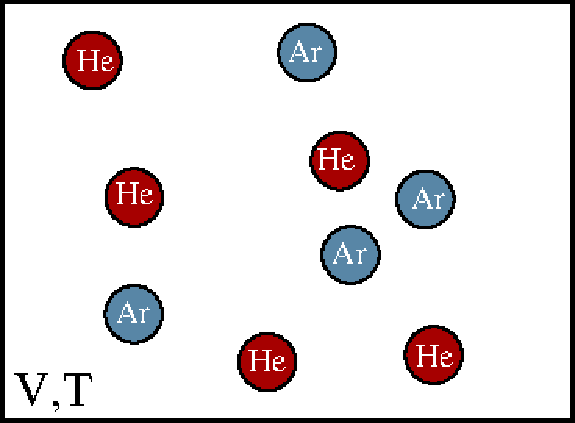
\includegraphics[width=0.5\textwidth]{mixing.pdf}\end{center}

\begin{enumerate}[label={(\alph*)}]
  \item What is the canonical partition function of the ($N_1 + N_2$)-particle mixture?

  \showmarks{4}

  \item Approximating $\displaystyle \log\left(N!\right) \approx -N \log\left(\frac{e}{N}\right)$, what is the Helmholtz free energy of the mixture?

  \showmarks{4}

  \item What is the internal energy $\vev{E}$ of the mixture?

  \showmarks{4}

  \item What is the entropy $S$ of the mixture?

  \showmarks{4}
\end{enumerate}
% ------------------------------------------------------------------



% ------------------------------------------------------------------
\section*{Question 2: Thermodynamic cycle}
An ideal gas in a container can access two different thermal reservoirs: a hot reservoir with high temperature $T_H$ and a cold reservoir with low temperature $T_L < T_H$.
The system carries out the thermodynamic cycle illustrated by the $PV$~diagram below, where the processes $A \to B$ and $C \to D$ are isothermal.
The five variables coloured red are given as inputs: The pressure $P_A$ at point $A$; The volume $V_A$ at points $A$ and $D$; The volume $V_B$ at points $B$ and $C$; The temperature $T_H$ at points $A$ and $B$; The temperature $T_L$ at points $C$ and $D$.

\begin{center}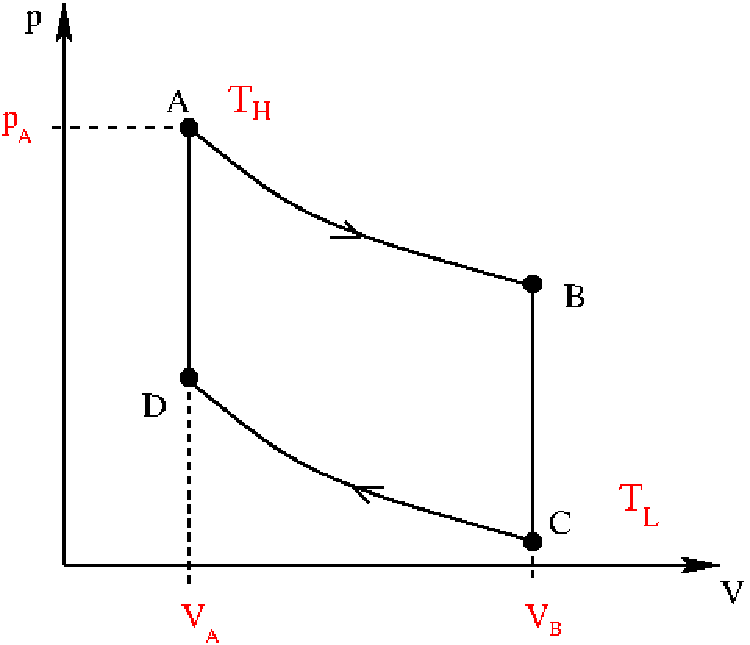
\includegraphics[width=0.5\textwidth]{cycle.pdf}\end{center}

\begin{enumerate}[label={(\alph*)}]
  \item Calculate the three unknown pressures $P_B$, $P_C$ and $P_D$ in terms of the input variables.

  \showmarks{6}

  \item How much work is done in each stage of the cycle?

  \showmarks{8}

  \item How much heat is exchanged in each stage of the cycle?

  \showmarks{8}

  \item What is the efficiency of the cycle?
        How does this efficiency compare to the efficiency of the Carnot cycle?

  \showmarks{6}
\end{enumerate}
% ------------------------------------------------------------------



% ------------------------------------------------------------------
\vfill
\section*{Question 3: Particle number fluctuations}
Starting from the average particle number for the grand-canonical ensemble,
\begin{equation*}
  \vev{N} = \frac{1}{Z_g} \sum_{i = 1}^M N_i \; e^{-\be (E_i - \mu N_i)},
\end{equation*}
derive a relation between $\displaystyle \pderiv{}{\mu} \vev{N}$ and the fluctuations $\vev{\left(N - \vev{N}\right)^2}$.

\showmarks{6}
% ------------------------------------------------------------------



% ------------------------------------------------------------------
\end{document}
% ------------------------------------------------------------------
